%!TEX root = main.tex

% \nathan{I think you need to better define what you mean by "primitive". Its usage is a bit confusing}
% \jeffrz{Don't explain what you're going to present, just tell me what you did! Also, "method" is a weird heading.}

% In this section, we will present in detail the different human intelligent tasks (HITs)
% of three primitives, and the computations that drive them.  We will
% also describe a backbone algorithm that is used to flexibly connect different
% primitives to form a complete workflow.  In the Experiment Sections we will show
% the results of three workflows that consist of different combinations of these
% primitives.

The Alloy system clusters a collection of clips, or short text descriptions (Figure~\ref{fig:phase1-example}), using a machine learning backbone that gathers various judgments from human workers. In our terminology, each human task is a ``Cast'' for human judgements which are then ``Gathered'' together with the machine learning backbone. Alloy enables Casts (here, crowdworker tasks) of different types and in different orders to be fused together by calling a Gather after each one. In each Cast stages, arbitrary number of workers can be hired for better robustness or lower cost. In this chapter, we present three types of Casts with different purposes as well as one type of Gather. At a high level, the ``Head Cast'' is aimed at finding common categories in the head of the distribution, while the ``Tail Cast'' is aimed at classifying categories in the tail of the distribution for which machine clustering has low confidence. The ``Merge Cast'' aims to clean up existing categories by combining highly similar categories. We also describe a Gather Backbone that fuses the judgements from multiple crowdworkers,
and connects multiple casts to form complete workflows. For ease of exposition we introduce each component in the context of a typical workflow: the Head Cast, the Gather, the Merge Cast, and the Tail Cast.


% We will now describe in detail how we elicit different types of human judgements
% to iteratively organize different parts of a dataset. The Head Cast captures salient
% keywords to uncover prominent categories that covers the head of the distribution. The Merge Cast cleans up
% existing categories by
% identifying duplications and combining them to form coherent structures. Finally, 
% the Tail Cast cleans up the remaining clips and identifies small categories to cover the tail of the distribution.
% We will also describe a Gather Backbone that fuses the judgements from multiple crowdworkers,
% and connects multiple casts to form complete workflows.
% In the following subsections, we will introduce them in the general order of actual workflows:
% Head Cast, Gather Backbone, Merge Cast, and Tail Cast.


\begin{figure}
	\centering
	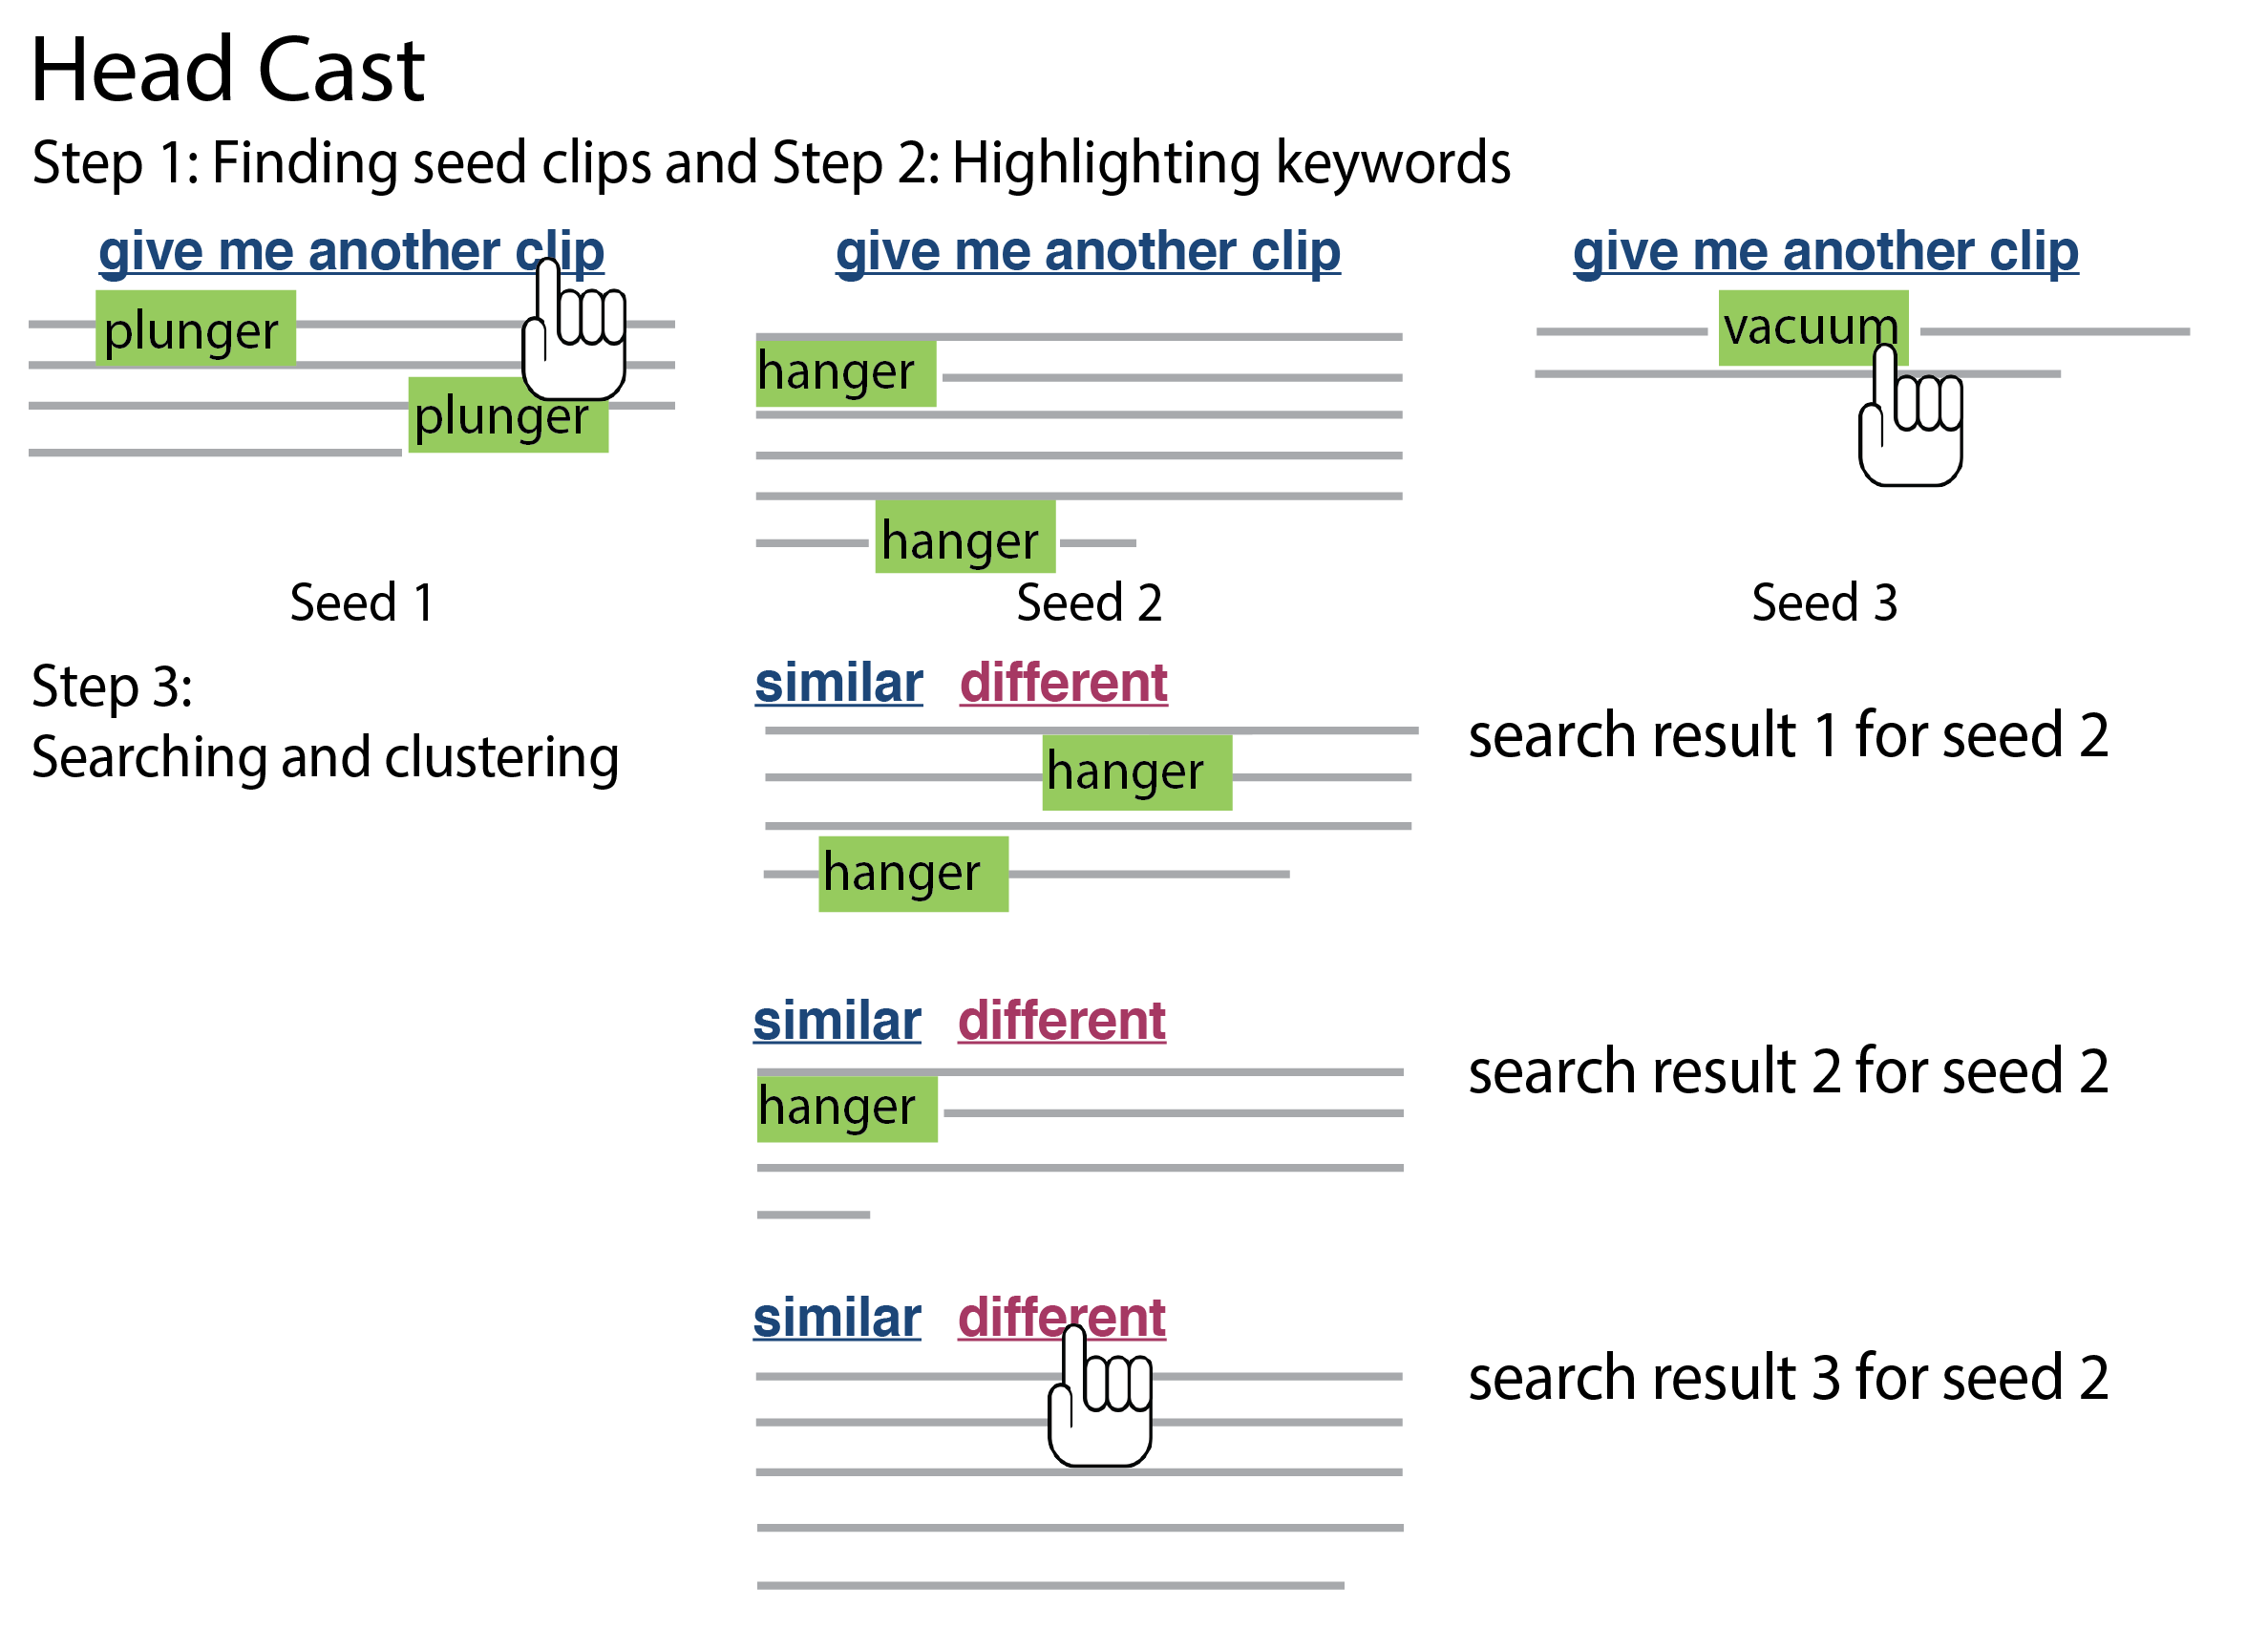
\includegraphics[width=0.6\columnwidth]{Chapters/Alloy/images/clusteringv2-04.png}
	\caption{The interface and steps of the Head Cast HIT.}
	\label{fig:phase1-hit}
\end{figure}

\subsection{The Head Cast}
The Head Cast aims to identify salient keywords to uncover the most common
categories in the head of the distribution. Doing so involves challenges in
providing workers sufficient context to know what a good category is, and also
in how to structure their work process in order to train a machine learning
algorithm to take over the classification of categories based on
human-identified seeds and keywords. 
Previous studies show that presenting multiple items from a collection can help
provide context to human workers \cite{medlin1978}, increasing the likelihood
of obtaining better clusters.  However, it can be difficult to determine how
much context is sufficient and how to produce a good sample that captures the
distribution of information of the whole dataset. 
Therefore, we introduce a new crowd-pattern we call ``\emph{sample and
    search}'' for providing global context through active sampling and
searching with keywords.   We ask crowdworkers to identify coherent categories
by presenting with four random items, but allowing them to replace each item by
random sampling from the entire dataset until they are confident that the items
will be in different categories in the final output.  This requirement gives them
the motivation to build up better global understanding of the dataset through
repeated sampling. After obtaining the four seed items, we ask crowdworkers to
identify keywords in each clips to search for related items in the dataset.
This process takes advantage of people's capacity of finding new information
\cite{pirolli1999information}. To create a familiar experience, we allow the
workers to freely change their query terms and update the search results in real
time. This way they can refine their searches based on the results, the same
way as when conducting online information foraging tasks \cite{jansen2009patterns}.
As shown in Figure~\ref{fig:phase1-hit}, the Head Cast HIT interface consists of three steps:

% The intuition is that a few keywords can be sufficient to
% identify important clusters in the head of the distribution
% \cite{huang2006text}. However, identifying important
% clusters and their salient words often requires a deep understanding of the
% data.

%The goal of Head Cast is to make use of human judgements to identify a set of
%keyword features and train an SVM model to partially cluster the given
%dataset \niki{this is a confusing way to introduce the SVM, since people will think you %are using it for clustering but you are using it more as a feature selection/similarity %metric enabler}.  Since it is infeasible to ask a crowdworker to organize the entire
%collection due to its size, each crowdworker
%worked on a small part of the dataset.  
% We implemented a three-stage workflow that uses machine learning models to augment initial human judgments.

%First, we use crowd workers to
%identify important topics and keywords through an interactive interface (Stage 1). Next we train an %SVM model to find the best set of features for predicting pairwise similarity of items based on the %human judgments (Stage
%2). Finally, we use those similarity judgments to create clusters using a
%hierarchical clustering backbone (Stage 3).

%\nathan{I changed the wording up here a bit}


% \jeffrz{***** If I were you, I'd make this two stages: stage 1 - human clustering, stage 2 - training and running an ML algorithm. this way you can echo the two-stage thing from the DESIGN section and reduce some redundancy}
% \joseph{two-phase actually refers to Head Cast and Tail Cast, not the steps here.}

% \subsubsection{Stage 1. Partial clustering and keyword extraction}

%Each crowdworker processes a
%portion of the input dataset using a set of four random seed clips we initially assign. 
%The idea is that most people are
%capable and familiar with picking out good keywords for retrieving documents
%through search. \nathan{maybe cite an IR paper about successful keyword search}.
%By asking crowdworkers to identify keywords in a seed clip to
%search for other clips that should be in the same category, we can record the
%process and gather not only clustering labels but also good feature dimensions
%at the same time.


\begin{enumerate}
    \setlength\itemsep{-1mm}

	\item \textbf{Finding seeds}:
    	Four random seed clips are presented to each crowdworker. Over each clip,
    	there is a button that allows them to replace the clip with another
    	random clip from the dataset.
		They are then asked to replace any clips
		that are too similar to the other seed clips.
		The workers repeatedly replace the seed clips
		until the four clips at hand belong to four different
		answer categories.
	\item \textbf{Highlighting keywords}:
	    The crowdworker is then instructed to highlight one to three
		unique keywords from each of the four seed clips that best identify
		their topics.  
	\item \textbf{Search and label}:
	    For each seed clip, we automatically search for
		similar clips from the entire corpus based on the highlighted keywords 
        and TF-IDF cosine similarity.
        The crowdworker is
		asked to label the top nine search results as \emph{similar} to or
		\emph{different} from their seed clips.
\end{enumerate}

% \niki{you need a rationale here; walk the reader through what problems you are solving with these steps so they can appreciate your solution.  Maybe reprupose stuff from the KA paper here, but you should adapt it so we don't get accused of plagiarism or something}

In Step 1, the crowdworkers need some understanding of the global context before
they can confidently judge that the seeds belong to different categories
in the final output. Previous work usually address this problem by presenting multiple
items to each crowdworker, in hopes of sampling both similar and dissimilar items
to give some sense of the global context. In reality it could be difficult to
judge how many items is sufficient for different datasets, and overly small size could lead to
bad samples that are unrepresentative of the global distribution.
We took a different approach by presenting fewer items at first,
but allowing workers to replace the seeds with random clips from
the dataset. This provide them both the mechanism and motivation to explore the dataset
until they have enough context to find good seed clips.

%The output of this stage is a number of potentially overlapping clusters, each
%contain one seed clip and nine other clips labeled as ``similar'' or
%``different''.

% unclear
%\begin{figure}[!h]
%	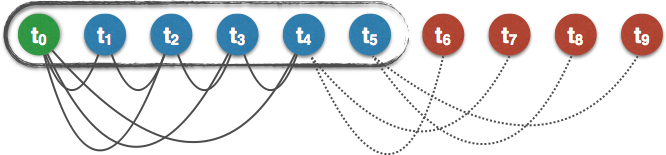
\includegraphics[width=0.9\columnwidth]{images/svm-clusters.png}
%	\caption{In Head Cast Stage1, crowdworkers create a cluster by selecting a
%		seed clip (green), and labeling 9 other clips as similar (blue) or
%		different (red). Each line connecting two clips indicates a training
%		events for Stage2.}
%	\label{fig:svm-clusters}
%\end{figure}

The intuition behind Step 2 is that people are already familiar with picking out good 
keywords for searching documents related to a concept via their online information
seeking experiences. In addition, requiring them to highlight unique keywords in the seeds
first, further ensures that they are familiar with the concepts in the seed clips, before
they search for similar items. In Step 3, the crowdworkers can still change and refine their
highlights from Step 2, and the system will refresh the search results in realtime. This
gives the crowdworkers both the motivation and mechanism to extract better keywords that lead
to better search results to label.
In Figure~\ref{fig:phase1-example}, we show two example clips from the datasets
collected using the two questions: \emph{How do I get my tomato plants to produce
more tomatoes?} and \emph{What does a planet need to support life?}
The highlighted words in each clips are the keywords selected by
one of the crowdworkers, showing that workers are finding useful words for classification.

%\niki{add rationale here about how this helps them in the next stage. you don't have to CALL it a design pattern since that's in KA, but give the intuition}

\begin{figure}
	\fbox{ \vbox{

		\ttfamily
        \scriptsize

% bad example
%		We had that problem too.  We snaked the bathroom tub, sink, \& stool so
%		many times.  The answer came to us when we had to replace the stool.
%		We found a \hilight{plumber} in the \hilight{yellow} \hilight{pages}.
%		Got some good recommendations.  They came and snaked the stack!  You
%		have to go on the roof for that.  If you can access the stack, rent as
%		big a plumber's snake as possible and to the job yourself.  Be sure to
%		ask the rental agency lots of questions, they want their equipment back
%		in good shape too. Be sure to clean the snaket (sic) off too.  That is
%		just plain common courtesy.  You will save lots of little tub snaking
%		jobs in the future
%
%		\rule{\columnwidth}{0.4pt}

		Tomato seedlings will need either strong, direct \hilight{sunlight} or
		14-18 hours under grow \hilight{lights}. Place the young plants only a
		couple of inches from florescent grow lights. Plant your tomatoes
		outside in the sunniest part of your vegetable plot.

		\rule{\columnwidth}{0.4pt}

        In its astrobiology roadmap, NASA has defined the principal
        habitability criteria as "extended regions of \hilight{liquid}
        \hilight{water}, conditions favourable for the assembly of complex
        organic molecules, and energy sources to sustain metabolism
	}}
	\caption{Example clips from two datasets with crowd keywords.}
	\label{fig:phase1-example}
\end{figure}


% \begin{figure}
% \footnotesize
% \hrule
% \vspace{2 pt}
% \textbf{Input:}\\
% \indent \ \ \ \ \ \ \ $S_{i,j}$: \ Sets of similar and different clips from Head Cast Stage 1\\
% \indent \ \ \ \ \ \ \ $K$: The set of all keywords from Head Cast Stage 1 \\
% \textbf{Output:} \\
% \indent \ \ \ \ \ \ \ \textit{Clusters}: Clusters of similar clips \\
% \indent \ \ \ \ \ \ \ \textit{Singletons}: Unclustered clips \\
% \textbf{Description:}
% \begin{algorithmic}[1]
% \STATE Let \textit{Sim} = \{$(t, t')$ $t, t' \in S_{i,j}$, $t, t'$ labaled "Similar"\}
% \STATE Let \textit{Diff} = \{$(t, t')$ $t$ labaled "Similar", $t'$ labaled "Different"\}
% \STATE \textbf{For} each $event_i \in$ \textit{Sim} $\cup$ \textit{Diff}:
%     \STATE \ \ \ \ \ \ Let $label_i$ = \textit{yes}, if $event_i \in$ \textit{Sim}, \textit{no} otherwise \\
%     \STATE \ \ \ \ \ \ Generate feature $feat_{i}$ based on $t, t', K$
% \STATE Train classifier \textit{M} using $label$, and $feat$
% \STATE \textit{Clusters}, \textit{Singletons} = HierchicalCluster($D$, $M$)
% \STATE \textbf{Return} \textit{Clusters}, \textit{Singletons}
% \end{algorithmic}
% \hrule
% \label{fig:phaseAstage2stage3}
% \caption{Pseudocode for Head Cast: Stages 2 and 3}
% \end{figure}

%\subsubsection{Stage 2. Similarity function: training an SVM model}

To learn a similarity function between clips, we use the crowd
labels and keywords to train a classifier that predict how likely two clips
to be labeled as similar.
Although the judgments from workers via the HIT interface about which clips go together provide valuable training information, we need to leverage these judgments to bootstrap similarity judgments for the clips that they did not label and to resolve potentially conflicting or partial category judgments. 
To do so we trained an SVM classifier in real-time to identify the set of keywords that are most indicative of categories and predict whether two clips in the dataset belonged to the same cluster.  
The training events
are all possible pairwise combinations of clips in the clusters obtained with the HIT interface,
which may include both positive (similar) and negative (different).
The feature dimensions are all the keywords highlighted by the
crowdworkers, and the value of each dimension is the product of
the number of times that keyword occurred in the two clips.
In general,  the keywords labeled by the crowdworkers contain little irrelevant information
compared to all words in the clips, but there could
still be some highlighted words that are not indicative of a category. For
example, one crowdworker worked on the dataset for ``\emph{How do I unclog my
	bathtub drain?}'' labeled ``\emph{use}'', ``\emph{a}'', and ``\emph{plunger}'' as
three keywords. Even though \emph{plunger} is a very
indicative feature for clustering this dataset, the first two highlighted words
seem too general to be useful. 
Using a linear kernel to
estimate the weights for the different dimensions (i.e., keywords) seems well suited for
our purpose \cite{chang2011libsvm, wu2004probability}.
Further, if the same keyword is used by different crowdworkers but lead to
very different labels, the linear SVM model will give lower weight to the corresponding dimention and
thus lower the effects of keywords that are less indicative of the categories.
We use LIBSVM which
implements a variant of Platt scaling to estimate probability 
\cite{lin2007note,platt1999probabilistic}. The overall intuition is that the SVM classifier is doing a form of feature selection, weighting those words in clips that could maximally distinguish clips amongst clusters. 
% \niki{I don't know if this is right, but you need to provide something like this as a rationale for each of your sections. Usually good to start with a problem you are trying to solve.}





% \jeffrz{do you need the rest of the stuff here? sounds too technical unless related work is important or reviewers complained last time}
% \joseph{this is from the reviewers last time (why is SVM needed / selected), i am shortening it by taking out the part with selecting bigram and trigrams.}
%This can potentially be solved by allowing turkers to extract
%bi-gram or tri-gram features from the clips, but it will also %increase interface
%complexity and decrease the coverage of the identified features %(e.g.,
%\emph{plunger} vs \emph{use a plunger}). On the other hand, a linear


In a preliminary experiment, we tested using all words in the clips as features to train
the SVM model. The intuition is machine algorithms might do a better job at identifying
keywords that can outperform keywords identified by crowdworkers. However, the results
show that using all words as features did not yield better results, and having much
higher feature dimensions increases the training time significantly.

%\subsubsection{Stage 3. Hierarchical clustering}
%\niki{is this actually the Gather stage? maybe integrate it into the bottom of the gather backbone section below?}

Finally, with the probability output of the SVM model 
as a similarity function between clips and a stopping threshold of $0.5$ probability,
we use a hierarchical clustering algorithm 
that serves as the Gather Backbone to capture head clusters. 

% We also tested different thresholds and found that 0.5 is the best performing condition overall. The output is a set of clustered and
% unclustered clips.

%\jeffrz{I have no idea what BACKBONE: HIERARCHICAL CLUSTERING means. make it more descriptive. (though I'd watch a movie titled that)}


\begin{figure}
	\centering
	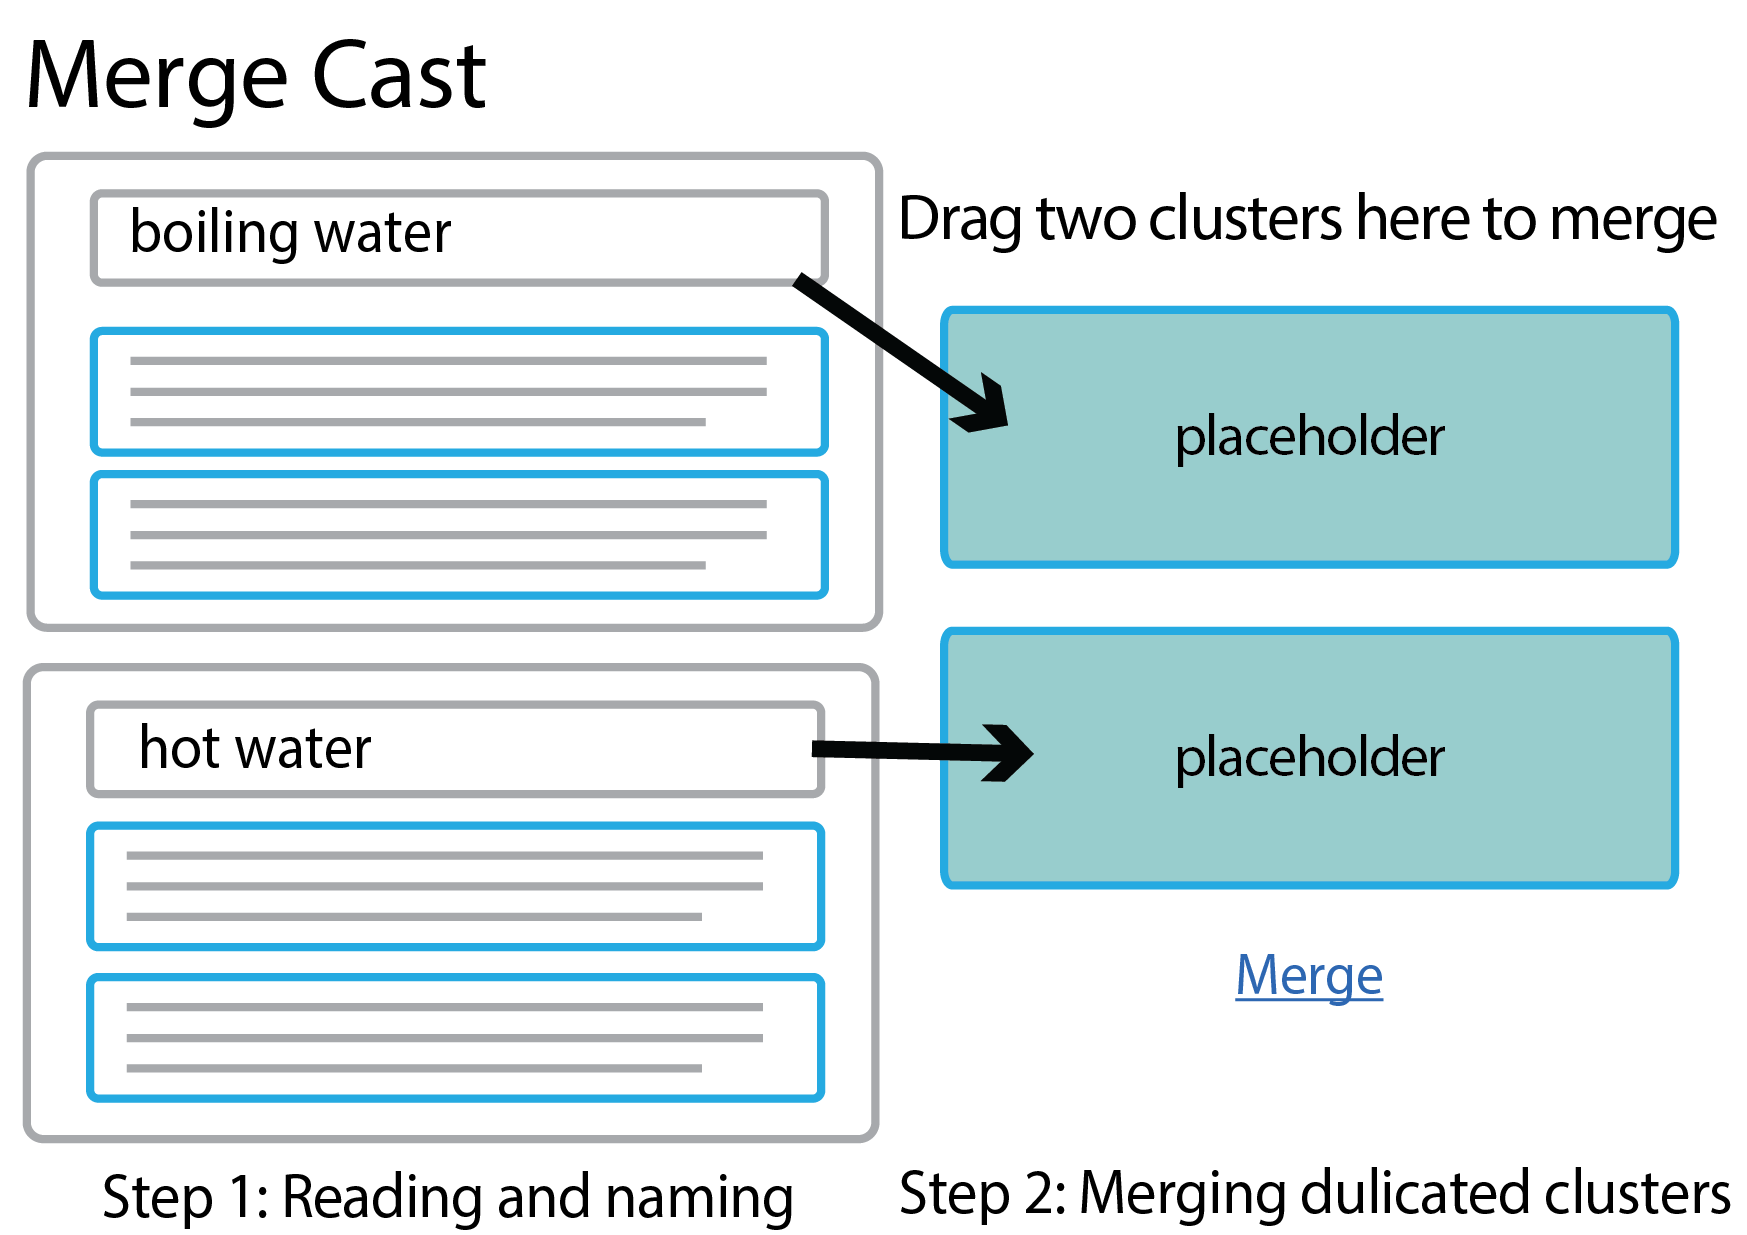
\includegraphics[width=0.47\columnwidth]{Chapters/Alloy/images/clusteringv2-02.png}
	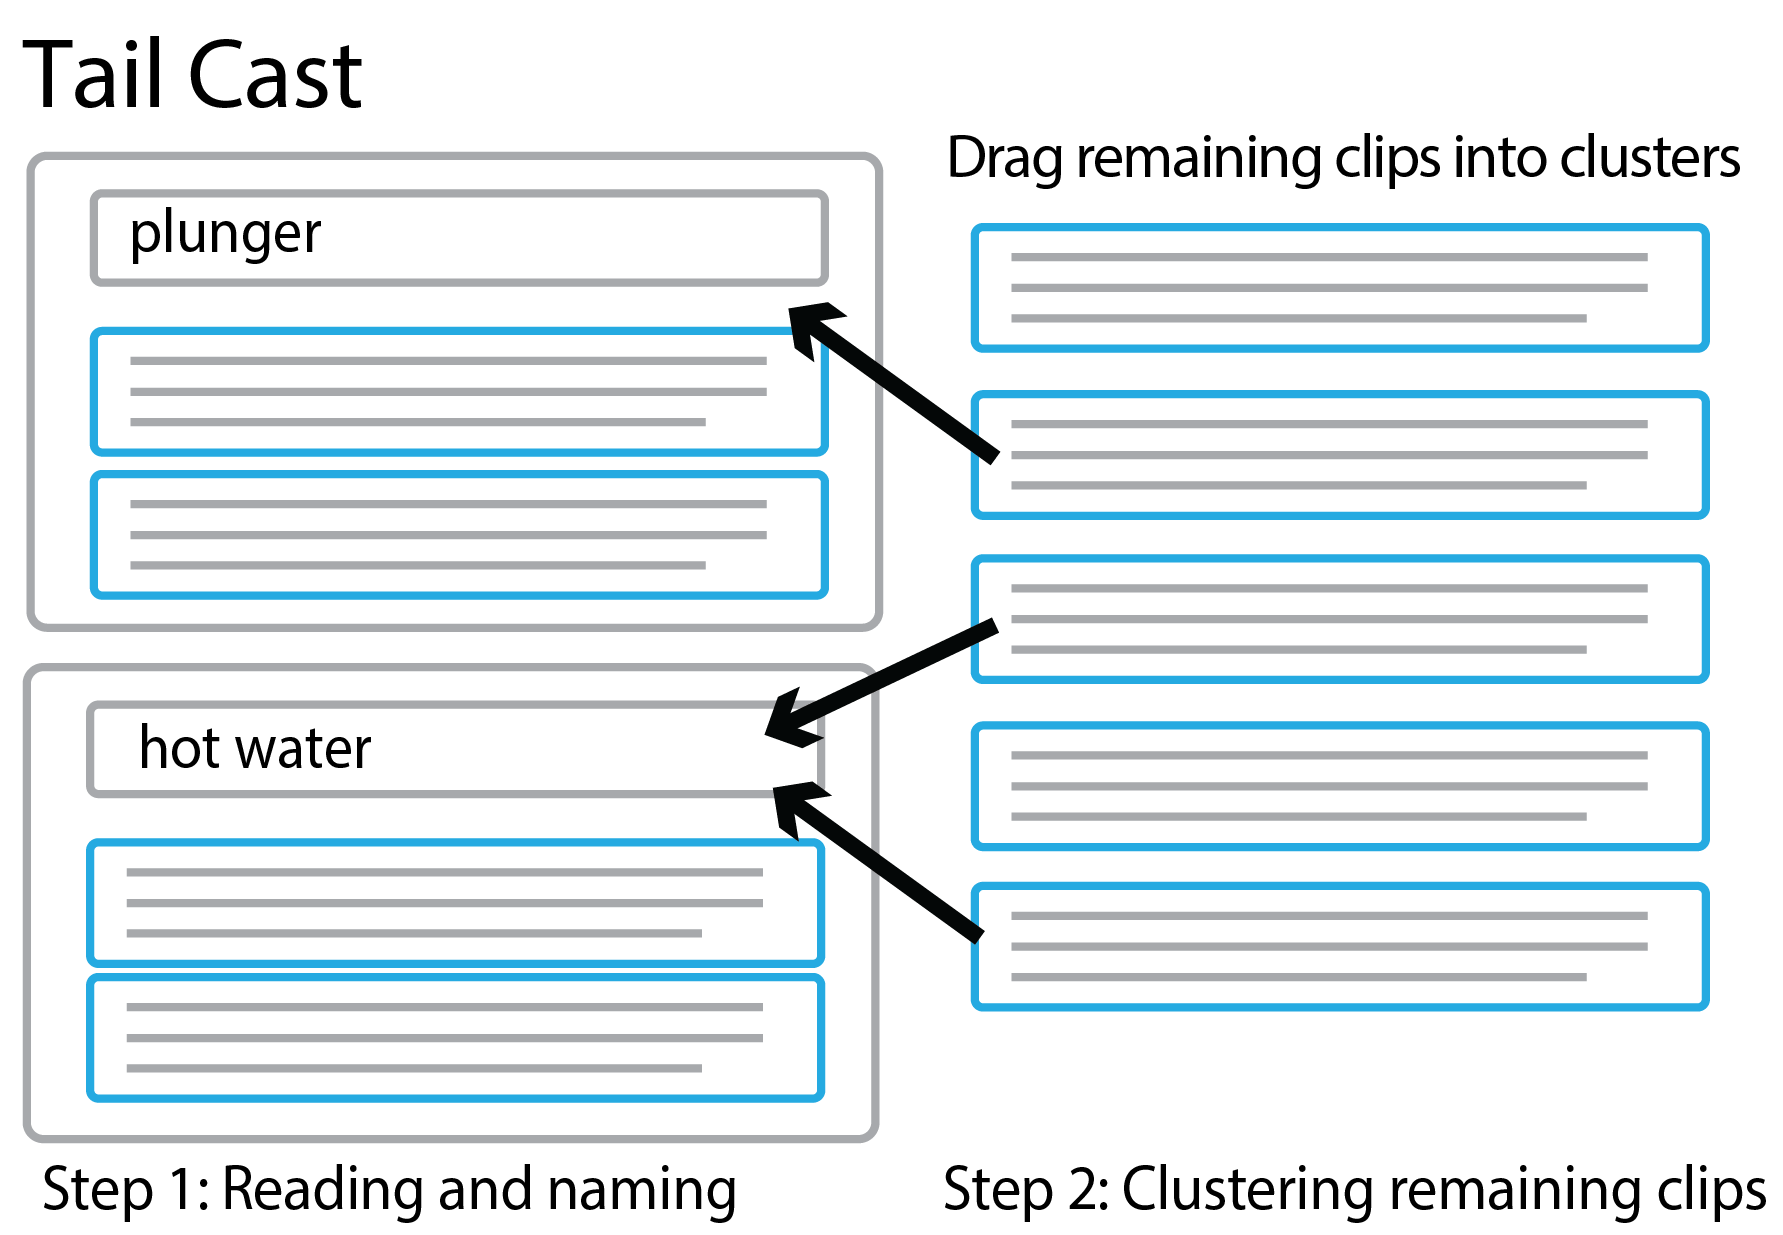
\includegraphics[width=0.47\columnwidth]{Chapters/Alloy/images/clusteringv2-03.png}
	\caption[HIT interface for the Merge Cast and the Tail Cast.]
        {The HITs for Merge Cast: Naming and merging existing
		clusters and Tail Cast: Clustering remaining clips.}
	\label{fig:phase2-hit}
\end{figure}

\subsection{Gather Backbone: Hierarchical Clustering}

\label{sec:hclustering}

%\jeffrz{I have no idea what primitives are now, and I am really, really lost. rewrite the two paragraphs as one}

Using a multiple-stage approach with different types of microtasks can make it
difficult to fuse together the different crowd judgements to form a coherent
result.  A key element to our approach in \textit{casting} for category
judgments in different ways is that we have a unifying mechanism to
\textit{gather} them back together.  For example, throughout our process we
cast for human category judgments in very different ways, including having
people identify seed clusters (the Head Cast), merge duplicated categories (the
Merge Cast), and classify the tail of the distribution (the Tail Cast).
Instead of creating ad-hoc links between these judgments we propose using a
unifying gathering mechanism composed of a machine learning backbone
which translates the different
\textit{casted} judgments into similarity strengths used as the basis of
clustering. We believe this \textit{Cast and Gather} pattern may be useful as
a way to conceptualize the relationship between machine algorithms and crowd
judgments for a variety of tasks.

% The Casts are designed to capture the varying types of human
% judgements that can be used to cluster different portions of the dataset. At
% different phases, the workflow iteratively creates new categories that cover
% more items in the dataset.

% remove candidate
To build a complete clustering workflow with multiple casts, we use a
hierarchical clustering algorithm as the backbone that connects different
casts. More specifically, the backbone algorithm  fuses the judgements
from different crowdworkers working on the same cast into
clusters, which, in turn, become the
shared context transferred to the next cast of the workflow.

With a clip similarity function from the prior cast and a stopping threshold, 
the hierarchical clustering method initially treats each clip as a
cluster by itself, and iteratively merges the two most similar clusters until a
threshold is reached. The result is a partially clustered dataset
with clusters and singletons. 
When the backbone is used after the last cast in the workflow, each
singleton is then merged into the most similar cluster.
The similarity between two clusters is defined as:

\vspace{-2mm}
\begin{equation}
	ClusterSim(\omega_1, \omega_2) = \frac{1}{|\omega_1||\omega_2|} \sum_{t_j \in \omega_1} \sum_{t_k \in \omega_2} ClipSim(t_j, t_k)
\end{equation}
\vspace{-1mm}

where $\omega_1$ and $\omega_2$ are the two clusters, $t_j$ and $t_k$ are each of the
clips in $\omega_1$ and $\omega_2$, respectively, and the $ClipSim()$ function is
the given similarity function between clips.


%\jeffrz{So we have Phase A, Consolidation Phase, and Phase B? I'm lost. Pick a "Phase" nomenclature and stick to it. I wouldn't do "Phase A", I'd give it a descriptive name kind of like you do here}
\subsection{The Merge Cast}
%\jeffrz{tighten this up. can you get by without "stages" and just paragraphs? you're losing lots of space on subheadings and nomenclature that may not be helpful unless it pops up again a few times in the paper}
%\niki{I would consistently go with "The Head Cast" instead of "Head Cast"}
While the Head Cast is designed to find the large clusters in the head of the
distribution, since each crowdworker works independently,
some of those clusters may actually
be different subsets of the same larger category or the same categories based
on different keywords (e.g., \emph{sunlight} vs \emph{natural lighting}).  The Merge Cast is designed to consolidate 
existing clusters by merging duplicated categories.  The input to this
cast is a set of clusters that may or may not cover the entire dataset,
and the output is fewer or equal number of clusters each with a list of ranked
short descriptions. 
The
challenge with detecting duplicate categories is that people need to understand
what is in each category first. 
We start by presenting a set of existing clusters, and asking crowdworkers to name 
each of them. This acts as a defensive design\cite{kittur2008crowdsourcing} that
ensures the crowdworkers
understand the current context (scope and abstraction level), and also to obtain
short descriptions for each of the clusters. 
Crowdworkers are
then asked to merge identical categories by dragging them into the
placeholders on the right (Figure~\ref{fig:phase2-hit}).

If there are too many head clusters to fit into a microtask,
the Merge Cast can be run recursively by
first running on disjoint sets of existing
clusters to consolidate them independently. Then, run another sets of
Merge Cast on the output of each initial Merge Casts, and recurse until
the output reduces to a set of clusters that
could be presented in a global Merge Cast to ensure consistency. 
The assumption here is that the set of clusters in the final output of Alloy should be
manageable by a single person to be useful.
We also wanted to point out that the number of clusters is likely to scale much slower than
the size of the dataset for many real-world data.
% In all six datasets we have tested, with up to 160 items, we have not encounter a case where we needed to run Merge Cast recursively.

% We can more formally characterize the scaling function as $T = log_c~N$,
% where $c$ represents the sparseness parameter of a dataset, $N$ the number of items 
% in the dataset, and $T$ the number of categories. The upper-bound limitation of 
% Alloy is then $T < L$, where $L$ is a limit on the complexity of a task given the characteristics of the 
% human computation platform utilized. Intuitively, this means that the Merge Cast will scale better 
% when the dataset involves fewer categories that explain more of the data, and when the human computation 
% platform supports more complex tasks.



With the labels from the crowdworkers,
we will again use the Gather Backbone to combine the judgements. The goal
is to merge existing clusters if more than half of the crowdworkers also
merged them in their solutions. Since in the Merge Cast
workers can not break up existing clusters or reassign clips, we can formulate 
the clip similarity function as:

\vspace{-2mm}
\begin{equation}
	ClipSim(t_1, t_2) = \frac{1}{N} |\{\omega: t_1, t_2 \in \omega \; and \; \omega \in \Omega\}|
\end{equation}
\vspace{-1mm}



where $t_1, t_2$ are the two clips, $N$ is the total number of crowdworkers,
$\Omega$ is the set of all clusters created by all crowdworkers, and $\omega$ is any cluster that contains both clips. This
function is robust against a few workers doing a
poor job. For example, if one crowdworker assigned every clip in the dataset to
a single, general cluster (e.g., \emph{answers}), the effect to the similarity function
would be equivalent to having one less crowdworker and applying Laplacian smoothing.
It is a common concern for crowd-based clustering methods
that novice workers may create overly abstract categories (e.g., \emph{solutions} or
\emph{tips}), that covers
all items in the datasets.
With our approach,
it would require more than half of the workers to merge all items into a single cluster
to generate a single cluster in the output.

% redundant
% We use the similarity function with a threshold of 0.5 to perform hierarchical
% clustering as described in the previous subsection, which is the equivalent of
% merging existing clusters when more than half of the crowdworkers also merged
% them in their solutions.

% \subsubsection{Stage 3. Ranking Cluster Names}

From the output of the Gather Backbone, we rank the short descriptions
associated with each cluster.
Since clips are labeled by multiple crowdworkers, each cluster
is associated with multiple
descriptions via its clips. We use the F1 metric to rank these names to
find the most representative description for each cluster, where the precision
of a name label is defined as
the number of clips in the cluster that it associates with divided by the size of the cluster,
and recall as divided by the total number of clips associated with it.

\subsection{The Tail Cast}

The Tail Cast is designed to clean up the remaining singleton clips by classifying
them into existing clusters or creating new clusters.  The intuition is that
even though machine learning techniques can produce high performance output,
sometimes it is achieved at the expense of sacrificing the border cases.
Human-guided ``clean up'' is often necessary for data produced by a machine
learning model.  The input of this cast is a set of existing clusters
(with or without short descriptions) and a set of remaining clips. The
output is a set of clusters with short descriptions.

We use an interface similar to the Merge Cast (Figure~\ref{fig:phase2-hit}),
and asked crowdworkers to review or name each of the existing clusters first,
so that they build up better global understanding of the dataset before they
organize the remaining clips. If Merge Cast was performed previously, their
names are presented to lower cognitive load.  The crowdworkers are then
instructed to cluster the unorganized clips shown on the right by assigning
them into existing clusters, creating new clusters, or removing uninformative
clips.  If there are too many remaining clips to fit into a single microtask,
they are partitioned into groups of 20 items.  Even though we may be dividing
the remaining clips into partitions, all workers in the Tail Cast starts with
learning the same global context that is the set of existing clusters from the
Head Cast.

%\subsubsection{Stage 1. Clustering with global constraint}

%\jeffrz{this is an example where the nomenclature gets to be a problem - I'm confused when you say "Phase B HIT". is it to make it different from a Phase A HIT? Why not give them more descriptive terms.}

% \subsubsection{Distributed Tail Cast}

% The amount of work in the Tail Cast is determined by both the size of the
% corpus and amount of clips covered by the Head Cast clusters.  It might not scale
% well if the size of the dataset increases.  For example, for a dataset of
% 200 clips, even if the Head Cast clusters cover 75\% of the items, the
% remaining 50 clips are still too many for a single crowdworker to organize in
% one HIT.
% Therefore, for datasets with more than 100 items, instead of showing all
% remaining clips to a single crowdworker, we distribute them across
% different HITs to different crowdworkers so that each crowdworker only work on
% 20 items. The idea is that even though they only see a small portion of the dataset,
% they are still organizing them based on the same existing context that is the
% Head Cast clusters.

%\subsubsection{Stage 2. Integrate clusters from multiple crowdworkers}
%\niki{aren't these just the Gather and then Merge Cast? rename if so?}

Finally, we use the Backbone Gather again to combine the multiple solutions
from the crowdworkers. The goal is analogous to the goal of the Merge Cast: if
two clips are assigned to the same category by more than half of the
crowdworkers, they should be in the same cluster in the combined solution.
For the similarity function, we simply replace the
variable $N$ in Equation~2 by the degree of redundancy.

% \begin{equation}
% 	\begin{split}
% 	ClipSim(t_1, t_2) & = \frac{1}{R} |\{\omega_j \forall t_1, t_2 \in \omega_j \; and \; \omega_j \in \Omega\}| \\
% 	                R & = \frac{20 * N}{|T|}
% 	\end{split}
% \end{equation}
% 
% where the redundancy $R$ is defined as number of HITs posted $N$, times the
% number of clips in each HIT $20$, divided by the number of remaining clips from
% Head Cast $|T|$.

% Finally, we can extract short descriptions for each cluster using the same
% F1 ranking described in the Merge Cast section.

% 
% \subsection{Time Complexity}

% \joseph{new}
% For each cast, we post different numbers of redundant HITs to Amazon Mechanical
% Turk. We can measure the time complexity by number of HITs posted in parallel.
% The time complexity for the Head Cast and the Merge Cast are $O(r_h)$ and
% $O(r_m)$ respectively, where $r_h$ and $r_m$ are the amount of redundancy.
% For the Tail Cast, the time complexity
% is $O(r_t  \lceil n / t \rceil)$, where $r_t$ is the amount of redundancy, $n$
% is the number of remaining items, and $t$ is the number of items presented to
% each crowdworker. In the Experiment Section, we will show the results of using
% different $r_h$ and $r_t$ on the same datasets to test the robustness of Alloy.



